\documentclass[10pt]{article}

\usepackage{listings}
\usepackage{graphicx}
\graphicspath{{artifact/images/}}

\pagenumbering{gobble}

\begin{document}

\title{A Novel Collaborative Filtering Algorithm by Bit Mining Frequent Itemsets}

\author{
Loc Nguyen \textsuperscript{1}, Phung T. M. Do \textsuperscript{2}\\
\textsuperscript{1} Sunflower Soft Company, An Giang, Vietnam\\
\textsuperscript{1} ng\_phloc@yahoo.com\\
\textsuperscript{2} University of Information Technology, Ho Chi Minh, Vietnam\\
\textsuperscript{2} dtminhphung@yahoo.com
}

\maketitle

\begin{abstract}
Collaborative filtering (CF) is a popular technique in recommendation study. Concretely, items which are recommended to user are determined by surveying her/his communities. There are two main CF approaches, which are memory-based and model-based. I propose a new CF model-based algorithm by mining frequent itemsets from rating database. Hence items which belong to frequent itemsets are recommended to user. My CF algorithm gives immediate response because the mining task is performed at offline process-mode. I also propose another so-called Roller algorithm for improving the process of mining frequent itemsets. Roller algorithm is implemented by heuristic assumption ``\textit{The larger the support of an item is, the higher it's likely that this item will occur in some frequent itemset}". It models upon doing white-wash task, which rolls a roller on a wall in such a way that is capable of picking frequent itemsets. Moreover I provide enhanced techniques such as bit representation, bit matching and bit mining in order to speed up recommendation process. These techniques take advantages of bitwise operations (\textit{AND}, \textit{NOT}) so as to reduce storage space and make algorithms run faster.

\textit{Keywords}: collaborative filtering; mining frequent itemsets; bit matching; bit mining
\end{abstract}

\section{Introduction}
Recommendation system recommends users favorite items among a large number of existing items in database. Items refer to anything such as products, services, books, and newspapers. It is expected that users are most interested in recommended items. There are two common trends: content-base filtering (CBF) and collaborative filtering (CF) in building up a recommendations system as follows \cite[pp.~3-13]{su:survey} \cite[pp.~73-139]{ricci:recommender}:
\begin{itemize}
\item The CBF recommends an item to user if such item has similarities in contents to other items that he like most in the past (his rating for such item is high). Note that each item has contents which are its properties and so all items will compose a matrix, called \textit{item content matrix}.
\item The CF, on the other hand, recommends an item to user if his neighbors which are other users similar to him are interested in such item. User's rating on any item expresses his interest on that item. All ratings on items will also compose a matrix, called \textit{rating matrix}.
\end{itemize}
Both CBF and CF have their own strong and weak points. CBF focuses on item contents and user interests. It is designed to recommend different items to different users. Each user can receive a unique recommendation and so this is a strong point of CBF. However CBF doesn't tend towards community like CF does.  If items that user may like ``are hidden under" his community, CBF is not able to discover such implicit items and so this is a weak point of CBF. Moreover, if the number of users is huge, CBF may give a wrong prediction whereas CF will get an increase in accuracy.

If there are huge contents associated with items, CBF will consume much more system resources and processing time in analyzing these items whereas CF does not encounter the problem of richness in item contents. CF only works on the user ratings of items instead, which is known as a strong point of CF. However, this also implies weak point of CF because CF can make unexpected recommendations in some situations, in which items are considered suitable to users but they do not relate to user profiles in fact. When many items are not rated, rating matrix is turned into \textit{spare matrix} which contains various missing values. The weakness of CF becomes more serious in case of spare matrix. There are two typical approaches to alleviate this weakness, as follows:
\begin{itemize}
\item The first one combines CBF and CF, called \textit{combination approach}. In typical scenario, the technique has two stages. Firstly, it applies CBF into completing spare matrix and secondly, it applies CF into making prediction for recommendation. The technique improves accuracy of prediction but it consumes much more time and resources because the first stage plays the role of pre-processing step and there is requirement of both item content matrix and rating matrix.
\item The second one compresses spare matrix into a \textit{representative model} which then is used to make recommendations. This is \textit{model-based approach} for CF. Note that CF has two common approaches such as memory-based and model-based. The model-based approach often applies statistical and machine learning methods into constructing representative model.
\end{itemize}
Although model-based approach does not give such a precise result as combination approach does, it can solve the problem of huge database and sparse matrix. Moreover it can respond user's request immediately by making prediction on representative model through instant inference mechanism. In general, there are four common approaches for model-based CF such as clustering model, latent model, Markov decision process model and matrix factorization model. Clustering CF \cite{ungar:clusteringcf} is based on the assumption that users in the same group have the same interest; so they rate items similarly. There are two clustering techniques: using clustering algorithms (\textit{k}-means, \textit{k}-centroids, etc.) and using Bayesian classifier. Authors \cite{miyahara:simplebayes} propose the Simple Bayesian Classifier for CF. Suppose rating values range in the integer interval \{1, 2, 3, 4, 5\}, there is a set of 5 respective classes \{$c_1$, $c_2$, $c_3$, $c_4$, $c_5$\}. The Simple Bayesian Classifier uses Naive Bayesian classification method \cite[p.~4]{miyahara:simplebayes} to determine which class a given user belongs to. Author \cite{langseth:bayescf} assumes that there is a linear mapping from the latent space of users and items to the numerical rating scale. Such mapping which conforms the full joint distribution over all ratings constructs a Bayesian network. Parameters of joint distribution are learned from training data, which are used for predicting active users' ratings. According to \cite{campos:hybridbayes}, the hybrid recommender model is the Bayesian network that includes three main kinds of nodes such as feature nodes, item nodes, and user nodes. Each feature node represents an attribute of item. Active users' ratings are dependent on these nodes.

Given a set of user $U$ = \{$u_1$, $u_2$,\ldots, $u_m$\} and a set of items $I$ = \{$i_1$, $i_2$,\ldots, $i_n$\}, observation ($u$, $i$) where $u \in U$ and $i \in I$ is considered as the co-occurrence of user and item. A latent class variable $c$ is associated with each co-occurrence ($u$, $i$). We have a set of latent class variables $C$ = \{$c_1$, $c_2$,\ldots, $c_k$\}. The mapping $c$: $U$ x $I$ $\rightarrow$ $C$ is called latent class model or aspect model \cite[pp.~91-92]{thomas:latentcf}. The problem which needs to be solved is how to specify the latent class model. Author \cite[p.~95]{thomas:latentcf} proposes Expectation Maximization (EM) algorithm to determine which latent variable $c \in C$ is the most suitable to be associated to ($u$, $i$).

Sparse rating matrix has insignificant rows or columns. Dimensionality reduction aims to get rid of such redundant rows or columns so as to keep principle rows/columns. As a result, the dimension of rating matrix is reduced as much as possible. Because this approach pays attention to analyzing matrix, it can be called matrix factorization approach. There are two well-known dimensionality algorithms such as singular value decomposition (SVD) and principle component analysis (PCA). Given rating matrix $M$, the SVD approach decomposes $M$ into three partial matrices $U$, $\Sigma$, $V$ so that $M$ is product of them, $M = U \Sigma V^T$ where the superscript \textit{T} denotes matrix transposition operation \cite[p.~1]{percy:svd}. $U$ and $V$ are called user feature matrix and item feature matrix, respectively. $\Sigma$ is diagonal matrix of eigenvalues. In study of CF, SVD is approximated by two ways \cite[pp.~2-5]{percy:svd}:
\begin{itemize}
\item Only $r$ largest eigenvalues are used to compose matrix $\Sigma$ and so matrices $U$, $\Sigma$, $V$ become smaller.
\item The objective function is established based on the sum of squared errors between existing ratings and predictive ratings. Matrices $U$, $\Sigma$, $V$ are parameters of such objective function. The gradient descent approach is used to adjust these parameters so as to minimize such objective function. This method is proposed by authors Simon Funk and Genevieve Gorrell. It is also called incremental SVD.
\end{itemize}

According to \cite[p.~1266]{shani:mdp}, recommendation can be considered as a sequential process including many stages. At each stage a list of items which is determined based on the last user's rating is recommended to user. So recommendation task is the best action that recommender system must do at concrete stage so as to satisfy user's interest. The recommendation becomes the process of making decision so as to choose the best action. Authors \cite[p.~1266]{shani:mdp} propose Markov decision process (MDP) to perform recommendation task. MDP is represented as four-tuple model \textless$S$, $A$, $R$, $T$\textgreater where $S$, $A$, $R$, and $T$ are a set of states, a set of actions, reward function, and transition probability density, respectively \cite[pp.~1270-1271]{shani:mdp}. The essence of making decision process is to find out the optimal policy with regard to such four-tuple model. Note that a policy is defined as the function that assigns an action to pre-assumption state.

In this paper, I aims to propose a new approach for model-based CF in which users' purchase patterns are mined and modeled as frequent itemsets which, in turn, are used to make recommendations. It is the efficient approach because it takes advantage of data mining \cite[pp.~227-250]{han:datamining}, leading to get fastest speed and high quality of recommendation. Among many researches focusing on model-based CF, the method to mine association rules for CF, proposed by authors \cite{shyu:associationrules}, is nearest to the CF algorithm in this paper. The authors \cite{shyu:associationrules} apply shortest path algorithm of graph theory into finding distances between web pages with note that these distances are derived from use access sequences. Association rules are mined based on such distances, then applied into CF.

The core of the proposed CF is bit mining to discover frequent itemsets, mentioned in section~\ref{section:roller}. It is required to do a survey on bit mining. The terms ``\textit{bit}" and ``\textit{binary}" have the same meaning in this paper.
Authors \cite{dong:bittablefi} propose so-called \textit{BitTableFI} algorithm. This algorithm uses data structure \textit{BitTable} to horizontally and vertically compress database for generating candidate itemsets and counting their supports in quick. Each row in BitTable, corresponding with a transaction in purchase database, is a string of bits and each bit (0 or 1) indicates whether or not an item is purchased.

Authors \cite{song:indexbittablefi} propose so-called \textit{Index-BitTableFI} algorithm which takes advantages of BitTable. According to \cite[p.~508]{song:indexbittablefi}, given a BitTable, index array and the corresponding computing method are proposed. By computing the subsume index, itemsets in accordance with representative item can be identified quickly through using breadth-first search at one time \cite[p.~509]{song:indexbittablefi}. Then, for the resulting itemsets generated by the index array, depth-first search strategy is used to generate all other frequent itemsets \cite[p.~510]{song:indexbittablefi}. Concept of index array is the core of Index-BitTableFI algorithm. This algorithm runs significantly faster than traditional BitTableFI algorithm.

BitTable and indexed BitTable contains fixed bit vectors. Alternately, authors \cite{vo:dbv-miner} proposed a Dynamic Bit-Vector (DBV) approach for fast mining frequent closed itemsets. Firstly, the authors \cite{vo:dbv-miner} used lookup table to calculate the support of itemsets fast. Secondly, the authors \cite{vo:dbv-miner} proposed subsumption concept to save memory and computing time. As a result, their approach is more efficient than CHARM algorithm in both the mining time and the memory usage \cite{vo:dbv-miner}.

Authors \cite{leon:compression} propose so-called \textit{AMFI} algorithm based on breadth first search through equivalence classes combined with compressed vertical binary representation of dataset \cite[p.~486]{leon:compression}. The binary representation and equivalence classes make the algorithm run faster. AMFI is not close to the bit mining in this paper because the essence of AMFI is to take advantages of breadth first search and equivalence classes.

Authors \cite{raja:bittablefi} propose so-called \textit{CPT-fi} algorithm following Apriori property but such algorithm clusters similar transactions into one and forms a \textit{compact bit-table} so as to reduce memory consumption and frequency of checking itemsets. Compact bit-table is the most significant aspect of CPT-fi algorithm \cite[p.~74]{raja:bittablefi}.

Authors \cite{kiraly:bittable} propose an Apriori-like algorithm but they take advantages of bit-table representation of dataset. Given two matrices of frequent itemsets, the algorithm takes Hadamard product of these matrices in order to generate candidate frequent itemsets \cite[p.~4]{kiraly:bittable}.

Authors \cite{li:slidingwindow} propose so-called \textit{MFI-TransSW} algorithm to mine frequent itemsets over online data streams with a \textit{transaction-sensitive sliding window}. The idea of sliding window is significant. The \textit{w}-length transaction-sensitive sliding window denoted \textit{TransSW} includes $w$ transactions. Given item $X$ is represented by a \textit{w}-length bit set. If $X$ is in the $i^{th}$ transaction, the $i^{th}$ of bit set of $X$ is set to be 1 \cite[p.~2674]{li:slidingwindow}. The MFI-TransSW has three phrases such as window initialization phrase, window sliding phrase, and frequent itemsets generation phrase \cite[p.~2674]{li:slidingwindow}. In the window initialization phrase, TransSW is created from coming transactions given pre-defined length $w$. The window sliding phrase is activated when TransSW is full. At that time, new coming transaction is added to TransSW and the oldest transaction is removed based on bitwise left shift operation. Finally, in the frequent itemsets generation phrase, MFI-TransSW algorithm uses bitwise operations to generate candidate itemsets and find frequent itemsets according to Apriori property \cite[p.~2675]{li:slidingwindow}.

Authors \cite{bashir:fast} build up lexicographic tree of items in transaction database. Itemset generation is done according to lexicographic order and bit-vector representation with attention that transaction database is transformed into bit table \cite[p.~8]{bashir:fast}. In a vertical bit-vector representation, if item $i$ is in transaction $j$, the bit $j$ of bit-vector $i$ is set to be 1. Moreover, the authors \cite[pp.~9-10]{bashir:fast} propose a so-called \textit{Projected-Bit-Regions} (PBR) to gain efficient projection of bit-vectors for calculating supports of itemsets. PBR and lexicographic tree are significant aspects of the research, which leads to achieve high speed in mining frequent itemsets.

When compared with other researches on bit mining, the proposed heuristic mining algorithms is the simplest one in which there is no requirement of complex structure and complicated computation. In other words, its strong point is based on its simplicity, in which what we need to do includes rolling bit sets with bit operations. As a result, it gains high speed although it can lose some frequent itemsets. Note that bit mining serves CF application mentioned in section~\ref{section:newcf} and only optimal frequent itemset is used to generate recommendation list. So, it is not requisite for discovering all frequent itemsets in the most accurate way.

This paper consists of five sections. In section~\ref{section:newcf}, I propose a new model-based CF algorithm based on mining frequent itemsets. The heuristic mining algorithm is discussed carefully in the section~\ref{section:roller}. Section~\ref{section:evaluation} is the evaluation. Section~\ref{section:conclusion} is the conclusion. Note that terms such as ``rating matrix", ``dataset" and ``database" have the same meaning in this paper.

\section{A new CF algorithm based on mining frequent itemsets} \label{section:newcf}
Given rating vector $u$ = (\textit{item}~1 = 3, \textit{item}~2 = 5, \textit{item}~3 = 2) indicates that user $u$ rated on \textit{item}~1, \textit{item}~2 and \textit{item}~3 with values 3, 5 and 2, respectively. The proposed CF algorithm, based on mining frequent itemsets, consists of two following processes:
\begin{itemize}
\item \textit{Modeling process} is performed in offline mode, in which a set of frequent itemsets $S$ is mined from rating matrix.
\item \textit{Recommendation process}: whenever user $u$ requires recommended items, a frequent itemset $s$ is chosen from $S$ so that $s$ contains items 1, 2 and 3, for instance, $s$ = (\textit{item}~1, \textit{item}~2, \textit{item}~3, \textit{item}~5, \textit{item}~7). The additional items 5 and 7 are then recommended to user. This process is performed in online mode.

\end{itemize}
Although the modeling process consumes much more time than the recommendation one does, it is executed in offline mode and so it does not cause any negative time-consuming impact on recommendation process. However, a serious problem is raised when the frequent itemset $s$ = (\textit{item}~1, \textit{item}~2, \textit{item}~3, \textit{item}~5, \textit{item}~7) didn't indicate rating values assigned to items 1, 2, and 3. It is known that items 1, 2 and 3 are rated by values 3, 5 and 2, respectively in rating vector $u$. It means that rating vector $u$ and frequent itemset $s$ don't match exactly. This causes another hazard to predicting missing ratings. Concretely, it is impossible to estimate rating values for items 5 and 7. These problems will be solved by using a so-called \textit{bit transformation} technique.

For instance, a rating matrix, where its rows indicate users, its columns indicate items and each cell is the rating which a user gives to an item. Suppose the ratings range in integer interval \{1, 2, 3, 4, 5\} where 5-most favorite and 1-most dislike, the sample rating matrix is shown in table~\ref{table:rating.matrix}.
\begin{table}
\centering
\caption{Rating matrix}
\begin{tabular}{|l|c|c|c|c|} \hline
&\textit{Item} 1&\textit{Item} 2&\textit{Item} 3&\textit{Item} 4\\ \hline
\textit{User} 1&3&5&2&5\\ \hline
\textit{User} 2&3&5&2&5\\ \hline
\textit{User} 3&1&5&4&\\ \hline
\end{tabular}
\label{table:rating.matrix}
\end{table}
Each item is ``stretched" into 5 sub-items which are respective to 5 possible rating values \{1, 2, 3, 4, 5\}. Each sub-item is symbolized as $item\_j\_k$ carrying two binary-states 1 and 0, which indicates whether user rates on item $j$ with concrete value $k$. For example, the bit sub-item $item\_2\_5$ getting state 1 shows that user gave rating value 5 on item 2. Now the rating matrix is transformed into \textit{bit rating matrix} in which each cell is the rating of bit sub-item. If a cell gets state 0, there is no one giving a rating on such cell yet. The bit rating matrix is shown in table~\ref{table:bit.rating.matrix}.
\begin{table}
\centering
\caption{Bit rating matrix}
\begin{tabular}{|l|c|c|c|} \hline
&\textit{User} 1&\textit{User} 2&\textit{User} 3\\ \hline
\textit{Item}\_1\_1&0&0&1\\ \hline
\textit{Item}\_1\_3&1&1&0\\ \hline
\textit{Item}\_2\_5&1&1&1\\ \hline
\textit{Item}\_3\_2&1&1&0\\ \hline
\textit{Item}\_3\_4&0&0&1\\ \hline
\textit{Item}\_4\_5&1&1&0\\ \hline
\end{tabular}
\label{table:bit.rating.matrix}
\end{table}

The frequent itemset, which is extracted from bit rating matrix, carries a so-called bit form $s$ = ($item\_j_1\_k_1$, $item\_j_2\_k_2$,\ldots, $item\_j_m\_k_m$). Each element $item\_j\_k$, is defined as bit sub-item. Rating vector is also transformed into bit rating vector $u$ = ($item\_j_1\_k_1$, $item\_j_2\_k_2$,\ldots, $item\_j_n\_k_n$). Thus, it is completely simple to match the bit frequent itemset $s$ with the bit rating vector $u$. For instance, the rating vector $u$ = (\textit{item} 1 = 3, \textit{item} 2 = 5, \textit{item} 3 = 2) is transformed into $u$ = ($item\_1\_3$, $item\_2\_5$, $item\_3\_2$) whereas the bit frequent itemsets are $s_1$ = ($item\_1\_3$, $item\_2\_5$, $item\_3\_2$, $item\_4\_5$) and $s_2$ = ($item\_1\_1$, $item\_2\_5$, $item\_3\_4$). We find that itemset $s_1$ is matched most with $u$ and so, the additional item 4 in $s_1$ is recommended to user with predictive value 5.

Now the aforementioned problems are solved but my algorithm should be enhanced. Suppose that the number of frequent itemsets is huge and each itemset has also a lot of items. When we match rating vector with frequent itemsets, there will be a boom of combinations that may cause computer system to be collapsed or consume much processing time. Therefore, I propose an enhancement method for matching purpose, based on \textit{bit matching} technique.

\subsection{Bit representation and bit matching}
Suppose a rating vector or frequent itemset contains 4 items and each item has 5 possible rating values, I use the bit set whose length is $4 * 5 = 20$ bits so-called 20-\textit{length} bit set to represent such a rating vector or frequent itemset. The bit set is divided into many clusters or groups, for example, if each item has 5 possible rating values then each cluster has 5 bits. So each cluster represents a sub-item and the position of a bit in its cluster indicates the rating value of corresponding sub-item. If a cluster contains a bit which is set (bit 1), its corresponding sub-item is rated with the value which is the position of such set bit. Table~\ref{table:bit.representation} shows an example of bit set. Note that the bit set is similar to bit vector proposed by the authors \cite{dong:bittablefi}, \cite{song:indexbittablefi} and Dynamic Bit-Vector proposed by the authors \cite{vo:dbv-miner}.
\begin{table}
\setlength{\tabcolsep}{3.5pt}
\centering
\caption{Bit representation}
\begin{tabular}{|c|c|c|c|c|c|c|c|c|c|c|c|c|c|c|c|c|c|c|c|} \hline
0&0&1&0&0&0&0&0&0&1&0&1&0&0&0&0&0&0&0&0\\ \hline
\multicolumn{5}{|c|}{Cluster 1}&\multicolumn{5}{|c|}{Cluster 2}&\multicolumn{5}{|c|}{Cluster 3}&\multicolumn{5}{|c|}{Cluster 4}\\
\multicolumn{5}{|c|}{(\textit{item} 1 = 3)}&\multicolumn{5}{|c|}{(\textit{item} 2 = 5)}&\multicolumn{5}{|c|}{(\textit{item} 3 = 2)}&\multicolumn{5}{|c|}{}\\ \hline
\end{tabular}
\label{table:bit.representation}
\end{table}
For example, rating vector $u$ = (\textit{item} 1 = 3, \textit{item} 2 = 5, \textit{item} 3 = 2) is transformed into $u$ = ($item\_1\_3$, $item\_2\_5$, $item\_3\_2$) which is represented as $u$ = (00100 00001 01000 00000) having four clusters. The frequent itemset $s_1$ = ($item\_1\_3$, $item\_2\_5$, $item\_3\_2$, $item\_4\_5$) is represented as $s_1$ = (00100 00001 01000 00001). The frequent itemset $s_2$ = ($item\_1\_1$, $item\_2\_5$, $item\_3\_4$) is represented as $s_2$ = (10000 00001 00010 00000). In order to match $s_1$ (or $s_2$) with $u$, we need to do \textit{AND} bit-operation between $s_1$ (or $s_2$) and $u$.
\begin{itemize}
\item If ($s_1$ \textit{AND} $u) = u$ then $s_1$ matches with $u$.
\item Otherwise ($s_1$ \textit{AND} $u) \neq u$ then $s_1$ doesn't match with $u$.
\end{itemize}
When $s_1$ get matched with $u$, we do \textit{AND-NOT} operation, as to extract items which are recommended to users. Suppose, the recommended item is denoted $r\_item$:
\begin{center}
$r\_item$ = $s_1$ \textit{AND} (\textit{NOT} $u$) = (00000 00000 00000 00001)
\end{center}
From this bit set, it is easy to recognize that item 4 is recommended with predict value is 5 because the fifth bit of 4\textsuperscript{th} cluster is set.

As a result, my algorithm will consist of three following steps:
\begin{itemize}
\item \textit{Step~1}: Rating matrix is transformed into bit rating matrix.
\item \textit{Step~2}: Bit rating matrix is mined to extract frequent itemsets.
\item \textit{Step~3}: Rating vector and frequent itemsets are represented as bit sets. Bit matching operations are performed in order to find out the appropriate frequent itemset which is matched with rating vector. Basing on such frequent itemset, it is possible to determine which items are recommended. Moreover missing values of recommended items can be also predicted.
\end{itemize}

\subsection{Pseudo-code for new CF algorithm}
Let $D$, $B$, $S$ be rating matrix, bit rating matrix and the set of frequent itemsets, respectively. Let $matched\_itemset$ and $r\_item$ be matched itemset and recommended item, respectively. Let $bitset$(\ldots) and $count$(\ldots) be functions that transform item into bit set and counts the number of bit 1 (s) in bit set, respectively. Let $bit\_transform$ be the function which transforms rating matrix into bit rating matrix.\\
Let $mining\_frequent\_itemsets$ be the mining function which extracts frequent itemsets from bit rating matrix (see subsections \ref{subsection:bit.mining}, \ref{subsection:improvement.roller}). Following is the pseudo-code like C language for my CF algorithm with note that rating matrix $D$ and recommended item $r\_item$ are input and output of algorithm, respectively. Steps 1 and 2 are specified at code lines 1-2. Step~3 is specified at lines 3-14. Lines 3-12 express how to determine optimal frequent itemset denoted \textit{matched\_itemset}. Lines 13-14 express how to extract recommended items from \textit{matched\_itemset}.
\begin{lstlisting}[mathescape]
(01) B = bit_transform(D)
(02) S = mining_frequent_itemsets(B)
(03) matched_itemset = null
(04) max_count = -1
(05) For each s $\in$ S
(06)   bs = bitset(u) AND bitset(s)
(07)   If bs = bitset(u) &&
(08)       count(bs) > max_count then
(09)     matched_itemset = s
(10)     max_count = count(bs)
(11)   End If
(12) End For
(13) r_item = bitset(matched_itemset) AND
(14)          (NOT bitset(u))
\end{lstlisting}
The second step, mining frequent itemsets from bit rating matrix, is the most important since it is the core of the proposed CF algorithm. Therefore the question ``how to extract frequent itemsets from rating matrix" will be answered in section~\ref{section:roller}.

\section{Mining frequent itemsets} \label{section:roller}
My mining frequent itemsets method is based on the assumption: ``\textit{The larger the support of an item is, the higher it's likely that such item occurs in some itemset}". In other words, items with high support tend to combine together so as to form a frequent itemset. So my method is the heuristic algorithm called Roller algorithm. The basic idea is originated from white-wash task. Suppose you imagine that there is a wall and there is the dataset (rating matrix) containing all items. Such dataset is modeled as this wall. On the wall, all items are shown in a descending ordering of their supports; it means that the higher frequent item is followed by the lower frequent item. Moreover, we have a roller and we roll it on the wall, from item to item, with respect to the descending ordering. If an item is found, satisfied at a minimum support ($min\_sup$), it will be added to the frequent itemset and the rolling task is continued until there is no item that meets minimum support. In the next time, all items in this frequent itemset are removed from the wall and the next rolling task will be performed to find out new frequent itemset.

My algorithm includes four following steps:
\begin{itemize}
\item \textit{Step~1}: Computing the supports of all items and arranging these items on the wall, according to the descending ordering of their supports. Note that all items whose supports don't meet minimum support $min\_sup$ are removed from such descending ordering. The kept items are called the frequent items. Of course, the first item in this descending ordering gets maximum support.
\item \textit{Step~2}: The $i^{th}$ itemset $i=\overline{1,n}$ is initialized by the first item in this descending ordering. The support of $i^{th}$ itemset is initialized as the support of this first item. The current item now is the first item and it will be removed from descending ordering.
\item \textit{Step~3}: If there is no item in descending ordering, the algorithm will be terminated. Otherwise:
  \begin{itemize}
  \item If the current item is the last one, in descending ordering, then all items in the $i^{th}$ itemset are removed from the descending ordering and the number $i$ is increased by 1 ($i = i + 1$). Go back step 2.
  \item If the current item is NOT the last in descending ordering, then, the next item is picked and so the current item now is the next item.
  \end{itemize}
\item \textit{Step~4}:
  \begin{itemize}
  \item The support of the $i^{th}$ itemset denoted $support$($i^{th}$ $itemset$) is accumulated by the current item; it is the count of total transactions that contains all items in both the $i^{th}$ itemset and current item. If $support$($i^{th}$ $itemset$) is equal to or larger than minimum support, current item is added to the $i^{th}$ itemset.
  \item Go back step 3.
  \end{itemize}
\end{itemize}
Steps 3 and 4 are similar to white-wash task which ``rolls" the $i^{th}$ itemset modeled as the roller. After each rolling (each iteration), such itemset gets thicker with more items.

Let $I$ = ($i_1$, $i_2$,\ldots, $i_m$) and $S$ be a set of items and a set of frequent itemsets, respectively. Let $C$ = ($c_1$, $c_2$,\ldots, $c_n$) be the list of items whose supports meet minimum support ($min\_sup$) and are sorted according to descending ordering, $C \subseteq I$. Let $s_i$ be the $i^{th}$ itemset. Let $c$ be the current item. Let $filter\_minimum\_support$(\ldots) be the function that filters items whose supports are greater than or equal to minimum support. Let $sort$(\ldots), $first$(\ldots), $next$(\ldots), $last$(\ldots) be sorting, getting first item, getting next item, getting last item functions, respectively. Following is the pseudo-code like C language for Roller algorithm programmed as function $mining\_frequent\_itemsets$ with note that the set of items $I$ and the set of frequent itemsets $S$ are input and output of such function, respectively.
\begin{lstlisting}[escapechar=\%]
(01) C = filter_minimum_support(I)
(02) C = sort(C)
(03) i = 1
(04) While (C %$\neq$% %$\emptyset$%)
(05)   c = first(C)
(06)   %s\textsubscript{i}% = {c}
(07)   While (true)
(08)     If c = last(C) then
(09)       S = S %$\cup$% 
(10)       C = C / S
(11)       break
(12)     Else
(13)       c = next(C)
(14)       b = bitset(%s\textsubscript{i}%) AND bitset(c)
(15)       If count(b) %$\geq$% min_sup then
(16)         %s\textsubscript{i}% = %s\textsubscript{i}% %$\cup$% {c}
(17)       End If
(18)     End If
(19)   End While
(20)
(21)   i = i +1
(22) End While
\end{lstlisting}
According to step~1, all frequent items are sorted at code lines 1-2. The $i^{th}$ itemset is initialized at lines 5-6, according to step~2. Lines 8-11 express that if current item $c$ is the last one then, the $i^{th}$ itemset is completed and its items are removed from $C$, according to step~3. Line 13 expresses that the next item is picked and it becomes the current item, according to step~3. Line 14 aims to calculate the support of the $i^{th}$ itemset accumulated by the current item, according to step~4. Given lines 15-16, the current item is added to the $i^{th}$ itemset if it satisfies minimum support.

Although the Roller algorithm may ignore some frequent itemsets but it runs much faster than traditional mining frequent itemsets methods. Especially, Roller algorithm can be enhanced by using \textit{bit mining} technique.

\subsection{Bit mining} \label{subsection:bit.mining}
When rating matrix is transformed into bit rating matrix, item and itemset become cluster (sub-item) and bit set, respectively. The support of item or itemset is the number of bits whose values are 1 (s) in bit set. Given minimum support is 2, table 4 shows frequent items extracted from bit rating matrix shown in table 2.
\begin{table}
\centering
\caption{Frequent items given minimum support 2}
\begin{tabular}{|l|c|c|c|} \hline
&\textit{User} 1&\textit{User} 2&\textit{User} 3\\ \hline
\textit{Item}\_2\_5&1&1&1\\ \hline
\textit{Item}\_1\_3&1&1&0\\ \hline
\textit{Item}\_3\_2&1&1&0\\ \hline
\textit{Item}\_4\_5&1&1&0\\ \hline
\end{tabular}
\label{table:frequent.items}
\end{table}

In step~1, sub-items are sorted according to descending ordering of their supports and some sub-items not satisfying minimum support ($min\_sup$) are removed given the minimum support is 2. Now sub-items are represented as bit clusters: $Item\_2\_5$ = (111), $Item\_1\_3$ = (110), $Item\_3\_2$ = (110), $Item\_4\_5$ = (110).

In step 2, the first itemset $s_1$ is initialized as $Item\_2\_5$ that is the first item in the ordering.
\begin{center}
$s_1$ = (111) and $support$($s_1$) = $count$(111) = 3
\end{center}
Where $support$(\ldots) denotes the support of itemset and $count$(\ldots) indicates the number of bits whose values are 1 (s) in bit set (\ldots).

In step 3 and 4, sub-items (clusters) such as $Item\_1\_3$, $Item\_3\_2$ and $Item\_4\_5$ are picked in turn and all of them satisfy minimum support.
\begin{itemize}
\item Picking $Item\_1\_3$: $s_1$ = $s_1$ $\cup$ {$Item\_1\_3$} = (111) \textit{AND} (110) = (110) $\rightarrow$ $support$($s_1$) = 2.
\item Picking $Item\_3\_2$: $s_1$ = $s_1$ $\cup$ {$Item\_3\_2$} = (110) \textit{AND} (110) = (110) $\rightarrow$ $support$($s_1$) = 2.
\item Picking $Item\_4\_5$: $s_1$ = $s_1$ $\cup$ {$Item\_4\_5$} = (110) \textit{AND} (110) = (110) $\rightarrow$ $support$($s_1$) = 2.
\end{itemize}
Finally, the frequent itemset is $s_1$ = (110) which includes $Item\_2\_5$, $Item\_1\_3$, $Item\_3\_2$ and $Item\_4\_5$. We recognize that the bit set of frequent itemset, named $s_1$ is accumulated by frequent item after each iteration. This makes algorithm run faster. The cost of counting bit set and performing bit operations isn't significant.

\subsection{Improvement of Roller algorithm} \label{subsection:improvement.roller}
Roller algorithm may lose some frequent itemsets in case that some frequent items don't have so high support (they are not excellent items) and they are in the last of descending ordering. So they don't have many chances to join frequent itemsets. However they really contribute themselves into some frequent itemset because they can combine together to build up a frequent itemset but they don't make the support of such itemset decreased much. It is difficult to discover their usefulness. In order to overcome this drawback, the Roller algorithm is modified so that such useful items are not ignored.

So in step~3, instead of choosing the next item as the current item, we can look up an item whose support is \textit{pseudo-maximum} and choose such item as the current item. The concept of pseudo-maximum is defined later. The Roller algorithm is improved by modifying steps 3 and 4 as follows:
\begin{itemize}
\item \textit{Step~1} is the same to that of normal Roller algorithm.
\item \textit{Step~2} is the same to that of normal Roller algorithm.
\item \textit{Step~3}: If there is no item in descending ordering, the algorithm will be terminated. Otherwise:
  \begin{itemize}
  \item If the current item is the last one, in descending ordering, then all items in the $i^{th}$ itemset are removed from the descending ordering and the number $i$ is increased by 1 ($i = i + 1$). Go back step~2.
  \item If the current item is NOT the last in descending ordering, we look an item up in the ordering so that such item can combine via \textit{AND} bit-operation with $i^{th}$ itemset so as to form the new itemset whose support is maximum and satisfies minimum support. Such item called \textit{pseudo-maximum support} item is chosen as the current item if it exists. If it does not exist, the current item is null.
  \end{itemize}
\item \textit{Step~4}: The current item is added to the $i^{th}$ itemset if it is not null. Go back step~3.
\end{itemize}
Following is the pseudo-code like C language for improved Roller algorithm programmed as function \\$mining\_frequent\_itemsets$ with note that the set of items $I$ and the set of frequent itemsets $S$ are input and output of such function, respectively. Code lines 9-19 find out pseudo-maximum support item according to step~3. Code line 24 adds such item to the $i^{th}$ itemset.
\begin{lstlisting}[escapechar=\%]
(01) C = filter_minimum_support(I)
(02) C = sort(C)
(03) i = 1
(04) While (C %$\neq$% %$\emptyset$%)
(05)   c = first(C)
(06)   %s\textsubscript{i}% = {c}
(07)   C = C / {c}
(08)   While (true)
(09)     c = null
(10)     pseudo_maximum = -1
(11)     For each item d %$\in$% C
(12)       temp = bitset(%s\textsubscript{i}%) AND bitset(d)
(13)       If count(temp)%$\geq$%min_sup && 
(14)        count(temp)>pseudo_maximum then
(15) 
(16)         c = d
(17)         pseudo_maximum = count(temp)
(18)       End If
(19)     End For
(20) 
(21)     If c = null then
(22)       break
(23)     Else
(24)       %s\textsubscript{i}% = %s\textsubscript{i}% %$\cup$% {c}
(25)     End If
(26)   End While
(27)   S = S %$\cup$% 
(28)   C = C / S
(29) 
(30)   i = i + 1
(31) End While
\end{lstlisting}
The improved Roller algorithm take slightly more time than normal Roller algorithm for looking up \textit{pseudo-maximum support} item in step~3 but it can discover more frequent itemsets. So its accuracy is higher than normal Roller algorithm.

\section{Evaluation and Discussion} \label{section:evaluation}
As aforementioned in the introduction section, the most significant feature of the proposed algorithm is simplicity with rolling bit sets, which relates to bit representation. If rating values are decimal numbers, it is required to convert decimal numbers to integer numbers in use of the proposed algorithm. For example, if rating values range in real interval [0, 1] then, values 0.0, 0.5, and 1.0 are converted to 0, 50, 100, respectively given integer interval [0, 1, 2,\ldots, 100]. The bit representation reduces storage space. For instance, database needs at least 3*10*8 = 240 bits to store ratings for 3 items and 10 users because each value needs 1 byte = 8 bits whereas it is only required 3*10*5 = 150 bits with bit representation given integer interval \{1, 2, 3, 4, 5\}. In other words, saving storage space is a strong point of the proposed algorithm.

Database Movielens \cite{groupLens:movielens} is used for evaluation. It is divided into 5 folders, each folder includes training set over 80\% whole database and testing set over 20\% whole database. Training set and testing set in the same folder are disjoint sets. The system setting includes: Processor Intel(R) Celeron(R) Dual-Core CPU N3050 @ 1.60GHz, RAM 4GB, Microsoft Windows 10 Pro 2015 64-bit, Java 8 HotSpot (TM) 64-bit Server VM. My proposed algorithm, named \textit{GreenFall}, is compared to three other algorithms: neighbor item-based, neighbor user-based and SVD \cite[pp.~151-152]{ricci:recommender}. These algorithms are implemented upon the infrastructure \textit{Hudup}. Note that Hudup is a middleware framework for e-commercial recommendation software, which supports scientists and software developers to build up their own recommendation algorithms with low cost, high achievement and fast speed. Hudup is accepted by European Project Space, whose trial version is available at

http://www.locnguyen.net/st/products/hudup

Such algorithms follows pre-defined specifications so that evaluation mechanism of Hudup can test them according to standard metrics. There are 7 metrics \cite[pp.~19-39]{herlocker:evaluation} used in this evaluation: \textit{MAE}, \textit{MSE}, \textit{precision}, \textit{recall}, \textit{F1}, \textit{response time} and \textit{setup time}. Response time metric, which measures speed of online recommendation process, is calculated in seconds. Setup time metric, which measures time consuming of offline modeling process (training process), is calculated in seconds.

MAE and MSE, abbreviations of absolute and mean squared errors, are average absolute and squared deviations between predictive ratings and users' true ratings \cite[pp.~20-21]{herlocker:evaluation}. Hence MAE and MSE are predictive accuracy metrics. The less they are, the high accuracy is. They are calculated by equations (\ref{math:mae}) and (\ref{math:mse}) in which $n$ is the total number of recommended items while $p_i$ and $v_i$ are predictive rating and true rating of item $i$, respectively.
\begin{equation}
MAE = \frac{1}{n}\sum_{i=1}^{n}|p_i-v_i|
\label{math:mae}
\end{equation}
\begin{equation}
MSE = \frac{1}{n}\sum_{i=1}^{n}(p_i-v_i)^2
\label{math:mse}
\end{equation}
Precision, recall and F1 are quality metrics that measure the quality of recommendation list - how much the recommendation list reflects user's preferences. An item is relevant if its rating is larger than or equal to average rating. For example, within rating range \{1, 2, 3, 4, 5\}, the average rating is $3 = (1 + 5)/2$. The larger quality metric is, the better algorithm is. An item is selective if it is recommended to users. Let $N_r$ be the number of relevant items and let $N_s$ be the number of selective items. Let $N_{rs}$ be the number of items which are relevant and selective. According to equations (\ref{math:precision}) and (\ref{math:recall}), precision is the ratio of $N_{rs}$ to $N_s$ and recall is the ratio of $N_{rs}$ to $N_r$ \cite[p.~23]{herlocker:evaluation}. In other words, precision is probability that selective item is relevant and recall is probability that relevant item is selective. F1 is regular combination of precision and recall, given equation (\ref{math:f1}).
\begin{equation}
Precision = \frac{N_{rs}}{N_s}
\label{math:precision}
\end{equation}
\begin{equation}
Recall = \frac{N_{rs}}{N_r}
\label{math:recall}
\end{equation}
\begin{equation}
F1 = \frac{2*Precision*Recall}{Precision+Recall}
\label{math:f1}
\end{equation}
Table~\ref{table:evaluation.result.100K} shows evaluation result on database Movielens 100K containing 100,000 ratings of 943 users on 1682 movies. The setup time of neighbor item-based and user-based algorithms is zero because these algorithms are memory-based CF and they do not have internal modeling process.
\begin{table}
\setlength{\tabcolsep}{4pt}
\centering
\caption{Evaluation result on database Movielens 100K}
\begin{tabular}{|l|r|r|r|r|} \hline
&\textbf{Proposed}&Item-based&User-based&SVD\\ \hline
MAE&\textbf{0.7279}&0.5222&0.9430&0.5036\\ \hline
MSE&\textbf{1.1737}&0.6675&2.1895&1.0849\\ \hline
Precision&\textbf{0.1326}&0.0245&0.0013&0.0042\\ \hline
Recall&\textbf{0.0524}&0.0092&0.0005&0.0015\\ \hline
F1&\textbf{0.0740}&0.0131&0.0008&0.0022\\ \hline
Setup&\textbf{2.3532}&0&0&120.64\\ \hline
Response&\textbf{0.0058}&10.918&9.5586&0.0117\\ \hline
\end{tabular}
\label{table:evaluation.result.100K}
\end{table}

As a result, my algorithm is more effective than other algorithms when it gets high quality with metrics: precision, recall, F1. Its F1 metric is 5.6 times, 98.5 times, 34 times better than item-based, user-based, and SVD, respectively. The reason is that it makes recommendations based on frequent itemsets which represent users' interesting patterns. However its accuracy is lower than item-based and SVD with metrics: MAE and MSE. Its MAE metric is 1.4 times and 1.45 times worse than item-based and SVD, respectively. The reason is that it does not do arithmetic operations like addition and multiplication to estimate missing rating values. In general, accuracy is strong point of SVD. Author \cite{paterek:svdimprove} proposed three improved variants of SVD such as RSVD2 which adds of biases to the regularized SVD, SVD\_KNN which post-processes SVD with k-nearest neighbor similarity, and SVD\_KRR which post-processes SVD with kernel ridge regression. The author \cite[p.~42]{paterek:svdimprove} evaluates these variants on Netflix Prize database, which results out that the MSE of methods: basic SVD, RSVD2, SVD\_KNN, and SVD\_KRR are $0.9826^2 = 0.9655$, $0.9039^2 = 0.8170$, $0.9525^2 = 0.9073$, and $0.9006^2 = 0.8111$, respectively. Although Netflix Prize database is different from Movielens database, the evaluation result of author \cite{paterek:svdimprove} asserts the preeminence of SVD with regard to accuracy in recommendation. Therefore quality is just preeminence of my algorithm.

Moreover it runs much faster than other methods. It responses 1870 times, 1637 times, 2 times faster than item-based, user-based and SVD, respectively. It is not dominant over SVD in response time but its modeling process consumes least time according to setup time metric which is 51 times faster than SVD. It consumes less memory because storage capacity of frequent itemsets is insignificant whereas SVD requires a large amount of memory to store decomposed matrices. In fact, mining frequent itemsets is faster than learning decomposed matrices. Figure~\ref{figure:comparison100k} shows comparison between the proposed algorithm and SVD with regard to metrics MAE, F1, setup time, and response time given database Movielens 100K.
\begin{figure}
\centering
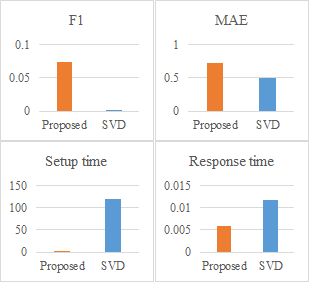
\includegraphics{Comparison100K.png}
\caption{Comparison between proposed algorithm and SVD given database Movielens 100K.}
\label{figure:comparison100k}
\end{figure}

When database is enlarged with much more ratings, given database Movielens containing 1,000,000 ratings (1M), memory-based CF algorithms like user-based and item-based can not run whereas the proposed algorithm and SVD keep their execution stable. The proposed algorithm is dominant over SVD in quality of recommendation and modeling process. Table~\ref{table:evaluation.result.1M} shows the evaluation result on database Movielens 1M.
\begin{table}
\setlength{\tabcolsep}{4pt}
\centering
\caption{Evaluation result on database Movielens 1M}
\begin{tabular}{|l|r|r|} \hline
&\textbf{Proposed}&SVD\\ \hline
MAE&\textbf{0.6231}&0.2550\\ \hline
MSE&\textbf{0.9790}&0.4208\\ \hline
Precision&\textbf{0.1048}&0.0029\\ \hline
Recall&\textbf{0.0342}&0.0009\\ \hline
F1&\textbf{0.0516}&0.0014\\ \hline
Setup&\textbf{23.405}&389.71\\ \hline
Response&\textbf{0.1152}&0.0946\\ \hline
\end{tabular}
\label{table:evaluation.result.1M}
\end{table}

Its quality via F1 metric is 37.08 times better than SVD whereas its accuracy via MAE metric is 2.44 times worse than SVD. Its setup time is 16.65 times faster than SVD while its response time is 0.82 times approximated to SVD. The reason is that it does bitwise operations on both offline modeling process and online recommendation process; the cost of these bitwise operations is low, regardless of database volume. Figure~\ref{figure:comparison1m} shows comparison between the proposed algorithm and SVD given database Movielens 1M. When comparing two evaluation results on database Movielens extended from 100K to 1M, recommendation quality is prominence of the proposed algorithm because its F1 scale is increased from 34 times to 37.08 times better than SVD. In general, the proposed algorithm is appropriate to fast and high quality recommendation applications when customers' purchase patterns are concerned most. It can mine frequent itemsets regardless of missing rating values and so, the problem of sparse matrix aforementioned in the introduction section is solved.
\begin{figure}
\centering
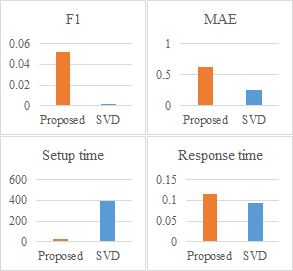
\includegraphics{Comparison1M.png}
\caption{Comparison between proposed algorithm and SVD given database Movielens 1M.}
\label{figure:comparison1m}
\end{figure}

\section{Conclusion} \label{section:conclusion}
My CF algorithm is different from other model-based CF algorithms when trying to discover user interests. The mining technique is important for extracting frequent itemsets considered as patterns of user interests. However traditional mining algorithms consume much more time and resources. So I proposed a new mining method, a so-called Roller algorithm. Based on evaluation measures, Roller is proved as reliable algorithm with high performance, fast speed, high quality of recommendation and consuming less time and resources. Its sole drawback is that it may ignore some interesting patterns because of heuristic assumption. However this drawback is alleviated by taking advantages of enhancement technique with the concept of pseudo-maximum support.

In the future, I will propose another model-based CF algorithm which applies Bayesian network into inferring user interests. Such algorithm based on probabilistic inference will be compared with the mining approach in this paper so that we have an open and objective viewpoint about recommendation study.

\section*{Acknowledgments}
This research is the place to acknowledge Sir Vu, Dong N. who gave me valuable comments and advices. These comments help me to improve this research.

\bibliographystyle{abbrv}
\bibliography{GreenFallCF}

\end{document}
